%% Creator: Inkscape inkscape 0.91, www.inkscape.org
%% PDF/EPS/PS + LaTeX output extension by Johan Engelen, 2010
%% Accompanies image file 'SessionComm.eps' (pdf, eps, ps)
%%
%% To include the image in your LaTeX document, write
%%   \input{<filename>.pdf_tex}
%%  instead of
%%   \includegraphics{<filename>.pdf}
%% To scale the image, write
%%   \def\svgwidth{<desired width>}
%%   \input{<filename>.pdf_tex}
%%  instead of
%%   \includegraphics[width=<desired width>]{<filename>.pdf}
%%
%% Images with a different path to the parent latex file can
%% be accessed with the `import' package (which may need to be
%% installed) using
%%   \usepackage{import}
%% in the preamble, and then including the image with
%%   \import{<path to file>}{<filename>.pdf_tex}
%% Alternatively, one can specify
%%   \graphicspath{{<path to file>/}}
%% 
%% For more information, please see info/svg-inkscape on CTAN:
%%   http://tug.ctan.org/tex-archive/info/svg-inkscape
%%
\begingroup%
  \makeatletter%
  \providecommand\color[2][]{%
    \errmessage{(Inkscape) Color is used for the text in Inkscape, but the package 'color.sty' is not loaded}%
    \renewcommand\color[2][]{}%
  }%
  \providecommand\transparent[1]{%
    \errmessage{(Inkscape) Transparency is used (non-zero) for the text in Inkscape, but the package 'transparent.sty' is not loaded}%
    \renewcommand\transparent[1]{}%
  }%
  \providecommand\rotatebox[2]{#2}%
  \ifx\svgwidth\undefined%
    \setlength{\unitlength}{589.08335571bp}%
    \ifx\svgscale\undefined%
      \relax%
    \else%
      \setlength{\unitlength}{\unitlength * \real{\svgscale}}%
    \fi%
  \else%
    \setlength{\unitlength}{\svgwidth}%
  \fi%
  \global\let\svgwidth\undefined%
  \global\let\svgscale\undefined%
  \makeatother%
  \begin{picture}(1,1.37291355)%
    \put(0,0){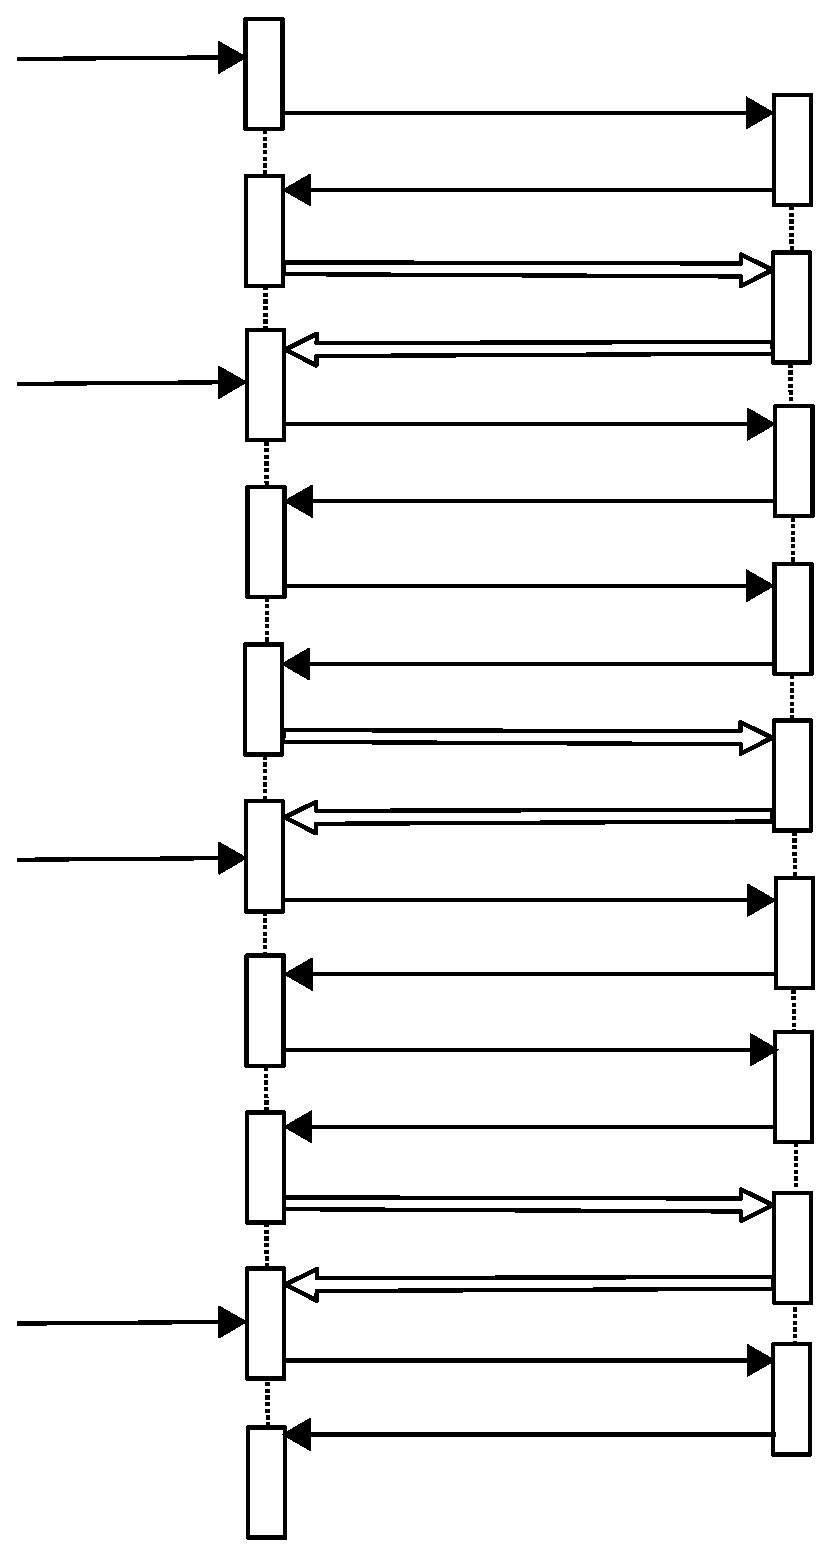
\includegraphics[width=\unitlength]{SessionComm.eps}}%
    \put(0.57353688,1.71009293){\makebox(0,0)[lb]{\smash{OK}}}%
    \put(0.53745431,1.8140856){\makebox(0,0)[lb]{\smash{Connect}}}%
    \put(0.57353688,1.315551849){\makebox(0,0)[lb]{\smash{OK}}}%
    \put(0.47506782,1.41783173){\makebox(0,0)[lb]{\smash{Set break-point}}}%
    \put(0.46847461,1.10916248){\makebox(0,0)[lb]{\smash{break-point hit}}}%
    \put(0.53745431,1.21035746){\makebox(0,0)[lb]{\smash{Continue}}}%
    \put(0.57353688,0.71916248){\makebox(0,0)[lb]{\smash{OK}}}%
    \put(0.19408814,1.9615099){\makebox(0,0)[lb]{\smash{\shortstack[lb]{Software\\subsystem}}}}%
    \put(0.86061571,1.9615099){\makebox(0,0)[lb]{\smash{\shortstack[lb]{FPGA\\prototype}}}}%
    \put(1.03781059,1.72241367){\makebox(0,0)[lb]{\smash{\shortstack[lb]{Establish connection}}}}%
    \put(1.03781059,1.30735925){\makebox(0,0)[lb]{\smash{\shortstack[lb]{Break-point set\\at  0xf0004010}}}}%
    \put(1.03781059,1.1148692){\makebox(0,0)[lb]{\smash{\shortstack[lb]{Execute instructions\\till  PC=0xf0004010}}}}%
    \put(1.03781059,0.12873744){\makebox(0,0)[lb]{\smash{\shortstack[lb]{Continue program\\ execution}}}}%
    \put(0.47506782,0.81512516){\makebox(0,0)[lb]{\smash{Set watch-point}}}%
    \put(1.03781059,0.72010607){\makebox(0,0)[lb]{\smash{\shortstack[lb]{Watch-point set\\ at 0xfffffffc}}}}%
    \put(0.53745431,0.62418622){\makebox(0,0)[lb]{\smash{Continue}}}%
    \put(0.46847461,0.52855633){\makebox(0,0)[lb]{\smash{watch-point hit}}}%
    \put(1.03781059,0.49992715){\makebox(0,0)[lb]{\smash{\shortstack[lb]{Execute instructions\\till memory access\\ at 0xfffffffc}}}}%
    \put(0.53745431,0.23902583){\makebox(0,0)[lb]{\smash{Detach}}}%
    \put(0.57353688,0.14619019){\makebox(0,0)[lb]{\smash{OK}}}%
    \put(0.4245431,1.52838723){\makebox(0,0)[lb]{\smash{Read processor state}}}%
    \put(0.4245431,0.94023407){\makebox(0,0)[lb]{\smash{Read processor state}}}%
    \put(0.4245431,0.3594973){\makebox(0,0)[lb]{\smash{Read processor state}}}%
    \put(-0.32292951,1.84515546){\makebox(0,0)[lb]{\smash{target remote}}}%
    \put(-0.34292951,1.4339728){\makebox(0,0)[lb]{\smash{Break at line 9}}}%
    \put(-0.28292951,0.84266105){\makebox(0,0)[lb]{\smash{Watch \textit{SUM}}}}%
    \put(-0.18292951,0.25072193){\makebox(0,0)[lb]{\smash{Detach}}}%
    \put(-0.24292951,1.99315099){\makebox(0,0)[lb]{\smash{User}}}%
  \end{picture}%
\endgroup%
